\chapter{Analyse de Fourier des systèmes à temps discret}
Dans le cas d'un signal périodique, la série de Fourier était utilisée
\begin{equation}
x(t) = \sum_{k=-\infty}^\infty a_ke^{jk\omega_0t}\qquad a_k = \frac{1}{T}\int_T
x(t)e^{-jk\omega_0t}
\end{equation}
où l'on peut voir $a_k$ comme le coefficient de pondération de chaque exponentielle 
complexe. Dans le cas ou les signaux n'étaient pas périodiques, la \textit{transformée 
de Fourier} (et inverse) a (ont) été définie(s)
\begin{equation}
X(j\omega) = \int_{-\infty}^\infty x(t)e^{-j\omega t}\ dt,\qquad x(t)=\frac{1}{2\pi}
\int_{-\infty}^\infty X(j\omega)e^{j\omega t}\ d\omega
\end{equation}
Le \textit{théorème de convolution} peut permettre un traitement plus aisé de la 
convolution
\begin{equation}
y(t) = x(t)*h(t)\qquad \ft\qquad Y(j\omega) = X(j\omega)H(j\omega)
\end{equation}

\section{Réponse à une exponentielle complexe}
Considérons l'entrée suivante
\begin{equation}
x(n) = z^n,\quad z=e^{j\omega_0}\qquad\Rightarrow\qquad x(n) = e^{j\omega_0n}
\end{equation}
où $-\infty<n<\infty$. Le signal de sortie est donnée en effectuant la convolution
\begin{equation}
\begin{array}{ll}
y(n) &= \sum_{k=-\infty}^\infty h(k)x(n-k) = \sum_{k=-\infty}^\infty h(k)z^{n-k} = z^n 
\underbrace{\sum_{k=-\infty}^\infty h(k)z^{-k}}_{H(z) \in \mathbb{C}}\\
&= H(z)z^n
\end{array}
\end{equation}
En effet, la dernière somme peut être vue comme une constante complexe (dépendant de $z$ 
et du SLP). Cette sortie  n'est que la fonction d'entrée multipliée par quelque chose : 
$z^n,z\in\mathbb{C}$ est une \textit{fonction propre} de tout SLP discret.\\
Si par hasard le signal d'entrée peut se mettre tous la forme d'une somme d'exponentielle 
complexe (fonction propre) multipliée par un scalaire
\begin{equation}
x(n) = \sum_p a_pz_p^n
\end{equation}
La réponse s'obtient par simple application de la linéarité
\begin{equation}
y(n) = \sum_p a_pH(z_p)z_p^n
\end{equation}
Ceci justifie l'analyse de Fourier pour les systèmes discrets.

\section{Série de Fourier discrète}
Il est possible de développer en série de Fourier un signal périodique (période $T_0$) 
à T\textbf{C} $x(t)$ 
\begin{equation}
x(t) = \sum_{k=-\infty}^\infty a_k e^{jk\frac{2\pi}{T_0}t}
\end{equation}
Il est dès lors tentant de vouloir faire de même pour un signal à T\textbf{D} périodique, 
de période $N$ ($x(n)=x(n+N)$) comme une combili d'exponentielle discrète de période $N$.\\
Nous avions vu qu'il n'existe que $N$ exponentielles discrètes distinctes de période $N$. 
C'est le cas ssi
\begin{equation}
\omega_0 = m\dfrac{2\pi}{N}\qquad m\in\mathbb{Z}
\end{equation}
La sommation est ainsi limitée à ces $N$ termes
\begin{equation}
x(n) = \sum_{k=0}^{N-1} a_ke^{jk\frac{2\pi}{N}n}\qquad n=0,1,\dots,N-1
\label{eq:syst}
\end{equation}
Il faut ainsi résoudre un système de $N$ équations à $N$ inconnues pour déterminer les $a_k$ 
d'une série $x(n)$ donnée :
\begin{equation}
\left\{\begin{array}{ll}
x(0) &= \sum_{k=0}^{N-1} a_k\\
x(1) &= \sum_{k=0}^{N-1} a_ke^{jk\frac{2\pi}{N}}\\
\dots\\
x(N-1) &= \sum_{k=0}^{N-1} a_ke^{jk\frac{2\pi}{N}(N-1)}
\end{array}\right.
\end{equation}

	\exemple{Déterminons la série de Fourier $x(n) = \sum_{k=0}^{N-1} a_ke^{jk\frac{2
	\pi}{N}n}\qquad n=0,1,\dots,N-1$ du signal ci-dessous (1,0,2,-1,\dots).
	\begin{center}
	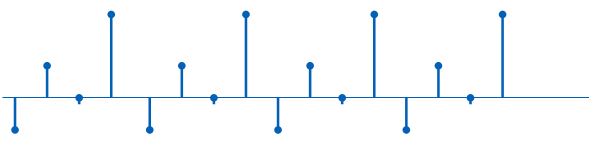
\includegraphics[scale=0.45]{ch3/image1.png}
	\captionof{figure}{ }
	\end{center}
	La série doit vérifier les points donnés, c'est-à-dire que le système ci-dessous 
	doit être satisfait.
	\begin{equation}
	\left\{\begin{array}{llll}
	x(0) &=1 &= \sum_{k=0}^{4-1} a_ke^{j2\pi k0/4} &= a_0+a_1+a_2+a_3\\
	x(1) &=0 &= \sum_{k=0}^{4-1} a_ke^{j2\pi k1/4} &= a_0+ja_1-a_2-ja_3\\
	x(0) &=1 &= \sum_{k=0}^{4-1} a_ke^{j2\pi k2/4} &= a_0-a_1+a_2-a_3\\
	x(0) &=1 &= \sum_{k=0}^{4-1} a_ke^{j2\pi k3/4} &= a_0-ja_1-a_2+ja_3		
	\end{array}\right.\quad\Leftrightarrow\quad\left\{\begin{array}{ll}
	a_0 &= 1/2\\
	a_1 &= -\frac{1+j}{4}\\
	a_2 &= -1\\
	a_" &= -\frac{1-j}{4}
	\end{array}\right.
	\end{equation}}

\newpage
Cette représentation n'est valable que si l'on peut exprimer les $a_k$ à partir de 
$x(n)$ : il faut résoudre le système de $N$ équations à $N$ inconnues \autoref{eq:syst}. 
Il faut pour cela calculer
\begin{equation}
\begin{array}{ll}
\displaystyle\sum_{n=0}^{N-1} x(n)e^{-jm\frac{2\pi}{N}n} &= \displaystyle\sum_{n=0}^{N-1}
\sum_{k=0}^{N-1} a_k e^{j(k-m)\frac{2\pi}{N}n}\\
&=\displaystyle \sum_{k=0}^{N-1} a_k \sum_{n=0}^{N-1} e^{j(k-m)\frac{2\pi}{N}n}
\end{array}
\end{equation}
La dernière somme peut être écrite
\begin{equation}
S = \sum_{n=0}^{N-1}x(n) e^{-j(k-m)\frac{2\pi}{N}n}  = \sum_{n=0}^{N-1} \alpha^n
\end{equation}
où $\displaystyle \alpha = e^{-j(k-m)\frac{2\pi}{N}}$. Il s'agit de la série géométrique
\begin{equation}
S = \left\{\begin{array}{ll}
N & \text{ si } \alpha = 1\quad \text{c-à-d si } k-m=0,\pm N,\pm 2N,\dots\\
\dfrac{1-\alpha^N}{1-\alpha} & \text{ si } \alpha \neq 1\quad \text{car } 
\alpha^N = 1
\end{array}\right.
\end{equation}
ou encore
\begin{equation}
S=\left\{\begin{array}{ll}
N &\text{ si } k-m = 0,\pm N, \pm 2N,\dots\\
0 &\text{ sinon}
\end{array}\right.
\end{equation}
Si $m\in[0;N-1]$, $S$ ne sera non nulle que pour $k=m$ et donc, en isolant
\begin{equation}
a_m = \frac{1}{N}\sum_{n=0}^{N-1} x(n)e^{-jm\frac{2\pi}{N}n}\qquad m=0,\dots,N-1
\label{eq:nouv}
\end{equation}
soit l'expression des coefficients de la série de Fourier discrète.


	\exemple{Reconsidérons le précédent exemple. Nous devrions retrouver les mêmes 
	coefficients à partir de \autoref{eq:nouv}. Nous avons ici
	\begin{equation}
	a_m = \frac{1}{4}\sum_{n=0}^{4-1} x(n)e^{-jm\frac{2\pi}{N}n} = \frac{1}{4}
	\left(1+2e^{-jm\pi}-e^{-jm3\pi/2}\right)
	\end{equation}
	On retrouve bien les mêmes coefficients.
	\begin{equation}
	\left\{\begin{array}{ll}
	a_0 &= 1/2\\
	a_1 &= -\frac{1+j}{4}\\
	a_2 &= -1\\
	a_" &= -\frac{1-j}{4}
	\end{array}\right.
	\end{equation}}\ \\
	
	
	\exemple{Pour le fun, calculons les coefficients de la série de Fourier de 
	$x(n) = \sin\left(\dfrac{2\pi}{N}n\right)$. On peut également écrire
	\begin{equation}
	x(n) = \dfrac{e^{j\frac{2\pi}{N}n}-e^{-j\frac{2\pi}{N}n}}{2j}
	\end{equation}
	La série de Fourier ayant la forme $x(n) = \sum_{k=0}^{N-1} a_ke^{j\pi kn/N}$, 
	en en déduit directement les coefficients par identification
	\begin{equation}
	a_1 = \frac{1}{2j},\qquad a_{-1} = -\frac{1}{2j},\qquad a_x=0\ \text{sinon}.
	\end{equation}}


\newpage
Ceci montre que $x(n)$ est intégralement (pfpfpf) défini par $N$ paramètres\footnote{
es $N$ valeurs du signal sur une période.} ; la série de Fourier discrète transforme 
ces $N$ paramètres en $N$ paramètres $a_k$. Nous utiliserons les notations suivantes 
(déplacement du facteur $1/N$) :
\begin{equation}
X(k) = \sum_{n=0}^{N-1} x(n)e^{-j\frac{2\pi}{N}nk},\qquad x(n) =\frac{1}{N}\sum_{
k=0}^{N-1} X(k)e^{j\frac{2\pi}{N}kn}
\end{equation}
où $X(k)$ ($=X(k+N)$) est la \textit{transformée de Fourier discrète} (DFT) de $x(n)$.\\
La linéarité appliquée en début de chapitre pour la sortie d'un SLP s'applique également 
ici de sorte que la sortie sera donnée par
\begin{equation}
y(n) = \frac{1}{N}\sum_{k=0}^{N-1} X(k)H\left(e^{j\frac{2\pi}{N}k}\right)
e^{j\frac{2\pi}{N}kn}\qquad \text{ où }\quad H\left(e^{j\frac{2\pi}{N}k}\right) = 
\sum_{k=-\infty}^\infty h(n)e^{-j\frac{2\pi}{N}kn}
\end{equation}
	
\section{Réponse en fréquence d'un système discret}
En considérant comme signal d'entrée discret $x(n) = e^{j\omega n}$, celle-ci étant 
fonction propre notre sortie sera
\begin{equation}
y(n) = H\left(e^{j\omega }\right)e^{j\omega n}
\end{equation}
où $\displaystyle H\left(e^{j\omega }\right) = \sum_{k=-\infty}^\infty h(k)e^{-j
\omega k}$ est la réponse en fréquence du système. Il s'agit d'une constante complexe 
pour $\omega$ fixé
\begin{equation}
H\left(e^{j\omega }\right) = \left|H\left(e^{j\omega }\right)\right|e^{j\text{arg} 
H\left(e^{j\omega }\right)}
\end{equation}
Dès lors, pour un signal d'entrée réel du type $x(n) = A\cos(\omega_0n+\varphi)$, la 
sortie vaut (superposition)
\begin{equation}
y(n) = A \left|H\left(e^{j\omega_0 }\right)\right|\cos\left(\omega_0n+\varphi+\text{arg} 
H\left(e^{j\omega n}\right)\right)
\end{equation}
On peut considérer $H\left(e^{j\omega}\right)$ comme le développement de la fonction 
périodique $H$ en série de Fourier. Dès lors, on peut exprimer les échantillons $h(k)$ 
par la formule classique de calcul des coefficients d'une série de Fourier
\begin{equation}
h(k) = \frac{1}{2\pi}\int_{-\pi}^\pi H\left(e^{j\omega }\right)e^{j\omega k}\ d\omega
\end{equation}
exprimant la réponse impulsionnelle en fonction de la réponse fréquentielle.


\exemple{Slide T32/34}
























